\documentclass[UTF8]{ctexart}

\usepackage{subfiles}  

%下面的语句, 引入你的头部设置文件
\usepackage{C:/phpStorm_proj/02_myself_ID_EGO/+100_latex_all_math_sel/myPreamble} 
%必须是绝对路径,才能让各个tex在单独编译时使用到

\title{文件名}


%---------------------------------


\begin{document}
	\tableofcontents % 生成目录
	\date{} % 若不写这句, 则默认也会渲染出日期, 所以我们要手动赋空值
	\maketitle  %这行代码, 让你前面的 title, author, date生效
	
	
	
	
	\part{数学期望 mathematic expectation}
	
	
	
	
	\section{加权平均数 : $		\overline{x}=\frac{\sum_{}^{}{\left( x\cdot \text{对应权重}w \right)}}{\sum_{}^{}{\left( \text{对应权重}w \right)}}		$}
	
	加权平均数, 和本章要讲的``数学期望", 没什么关系. 但两者的公式, 确有相似之处. 所以就把``加权平均数"也写在这里.\\
	
	若n个数$ x_1, x_2, ..., x_n$ 的``权重", 分别是 $ w_1, w_2, ..., w_n$ ,那么, 这n个数的``加权平均值"就是: \\
	$	\overline{x}=\dfrac{x_1w_1+x_2w_2+...+x_nw_n}{w_1+w_2+...+w_n}	$. 
	即: $		\overline{x}=\dfrac{\sum_{}^{}{\left( x\cdot \text{对应权重}w \right)}}{\sum_{}^{}{\left( \text{对应权重}w \right)}}		$ \\
	
	
	\begin{myEnvSample}
\begin{tabular}{|c|c|c|c|}
	\hline
	各考试 & 平时测验=得到了80分 & 期中考试=90分 & 期末考试=95分 \\
	\hline
	权重 & 0.2 & 0.3 & 0.5 \\
	\hline
\end{tabular} \\

则, 你成绩的``加权平均值" : \\
 $\overline{x}=\dfrac{\sum_{}^{}{\left( x\cdot \text{对应权重}w \right)}}{\sum_{}^{}{\left( \text{对应权重}w \right)}}=\dfrac{\left( 80\cdot 0.2 \right) +\left( 90\cdot 0.3 \right) +\left( 95\cdot 0.5 \right)}{0.2+0.3+0.5}=90.5$ 
	\end{myEnvSample}
	\vspace{1em} 
	
	
	
	
	
	
	
	
	\section{``期望" : 是对长期价值的数字化衡量.}
	
	各个股票的价格有涨有跌, 那你怎么判断它们各自的价值, 到底几何? 方法就是 --- 数学期望.  \\
	\textbf{``期望" 是对``长期价值"的数字化衡量. --- 即``长期中会得到的数学均值". 即在长期中(无数次试验)的状态下, 能取到的稳定结果(即均值)为何.} \\
	
	
	``数学期望"之所以有效, 是因为``大数定律"在背后起作用. \\
	- \textbf{大数定律把``随机变量x"在局部上的``随机性数值变化", 固定到``整体上的确定性",也就是概率.} \\
	- \textbf{而``数学期望", 又把``概率"代表的长期价值, 变成了一个具体的数字,方便我们比较.} \\
	
	几乎所有的金融产品的价值, 如基金, 股票, 都可以用``数学期望" 来衡量它们是否值得投资. 如果``赢的期望"超过``输的期望",即\textbf{数学期望是正的, 它就值得长期投资.} \\	
	对于游戏开发者来说, \textbf{如何保证游戏的平衡性?} 即不让某些游戏中的职业过强或过弱? \textbf{方法就是衡量每个角色职业能活下来的``数学期望". 然后调整参数, 达到``数学期望"上的平衡.} \\
	
	
	不过注意: 数学期望, 有时也会有``主观价值判断"的涉入. 因为每个人, 对同一样事物赋予的``价值高低"的判断不同, 所以不同个体的数学期望, 也不一样. 比如, 俄罗斯轮盘赌, 那些把赢钱看得比自己生命更重的人, 他们赋予这个游戏的数学期望就更高. 
	
	
	
	
	
	\section{``离散型"随机变量的``数学期望": $E(X)= \sum_{k=1}^{\infty} (x_k P_k)$}
	
	该公式的意思就是: 将该随机变量的一切可能的``取值", 各自乘以其对应的``概率", 然后将这些乘积``求总和". 如果该求和, 能得到一个``绝对收敛"的数, 那么这个收敛数, 就是该``离散型随机变量"的"数学期望E". 记为$E(x)$. \\
	它其实是简单算术平均的一种推广,类似``加权平均"。\\
	
	具体就是: \\
	离散型随机变量X 的取值为: $ X_1, X_2, ... X_n$, 其每个X的取值, 对应的概率为 $ p(X_1), p(X_2),..., p(X_n)$. 这些概率, 也可理解为数据 $ X_1, X_2, ... X_n$ 出现的频率 $ f(X_i)$. 则: \\
	$\boxed{
	X_1\cdot p(x_1)+X_2\cdot p(x_2)+...+X_n\cdot p(x_n)=\sum_{k=1}^n{(x_k \cdot p_k)}=\underset{\text{随机变量}X\text{的期望}}{\underbrace{E(X)}}
	}$ \\
	← 这个公式和``加权平均数"的公式很像, 只不过是把``权重"换成了``概率". \\
	
	
	
	
\begin{myEnvSample}
你在一游戏中, 要么会得到0元, 要么100元, 具体概率如下. 则你的期望为? \\
\begin{tabular}{|c|c|c|}
	\hline
	X(元) & 0 & 100 \\
	\hline
	P(概率) & 3/4 & 1/4 \\
	\hline
\end{tabular} \\

$E(X)=\sum_{k=1}^n{(x_k\cdot p_k)}=\left( 0\cdot \frac{3}{4}+100\cdot \frac{1}{4} \right) =25\text{元}$ 
\end{myEnvSample}
	\vspace{1em} 
	
	
	
	
	\begin{myEnvSample}
某股票, 现在价格50元. 它有40\%的概率涨到60块, 有30\%的概率保持不变, 还有30\%的概率跌到35块. 即: \\
\begin{tabular}{|c|c|c|c|}
	\hline
	收益 X(元)=未来价格-现在价格(50元) & =60-50 & =50-50 & =35-50 \\
	\hline
	P & 0.4 & 0.3 & 0.3 \\
	\hline
\end{tabular} \\

那么它未来涨跌收益 的``数学期望"就是:  \\
$E(X) = (60-50) \cdot 0.4 + (50-50) \cdot 0.3 + (35-50) \cdot 0.3 = -0.5$  \\
这个收益的期望, 是负数. 说明长期来看, 这只股票趋向于是亏钱的, 不值得买.
	\end{myEnvSample}
	\vspace{1em} 
	
	
	
	
	\begin{myEnvSample}
\begin{tabular}{|c|c|c|}
	\hline
	投篮得分X ↓ & ← 命中概率 & ← 数学期望 \\
	\hline
	近距离篮下投, 得2分 & 0.55 & 2×0.55=1.1分 \\
	\hline
	中距离投篮, 得2分 & 0.45 & 2×0.45=0.9分 \\
	\hline
	远距离投三分球, 得3分 & 0.35 & 3×0.35=1.05分 \\
	\hline
\end{tabular} \\

\textbf{每种进攻方式的价值, 原本没办法比较,有了``数学期望"后, 就可以进行比较了.} 所以要多采用``近距离"和``远距离"投篮 (因为它们的数学期望值更高), 少投"中距离". 事实上, 在NBA 篮球联赛中, 不少球队就是照这个思路制定策略的.
	\end{myEnvSample}
	\vspace{1em} 
	
	
	
	
	
	\begin{myEnvSample}
		某城市, 家庭中拥有孩子的数量, 是一个随机变量X, 取值为0,1,2,3. \\
		\begin{tabular}{|c|c|c|c|c|}
			\hline
			& 孩子数量X=0 & x=1 & x=2 & x=3 \\
			\hline
			概率 & P=0.01 & P=0.9 & P=0.06 & P=0.03 \\
			\hline
		\end{tabular} \\
	
	该城市的家庭, 孩子数量的期望就是: \\
$E(X)=\sum_{k=1}^n{(x_k\cdot p_k)}=(0\cdot 0.01)+(\underset{1\text{个孩子}}{\underbrace{1}}\cdot \underset{\text{概率是}0.9}{\underbrace{0.9}})+(2\cdot 0.06)+(3\cdot 0.03)=1.11$ 	
	\end{myEnvSample}
	\vspace{1em} 
	
	
	
	\begin{myEnvSample}
		有甲乙两人, \\
		- 甲会生产出``次品的数量"和``相应概率"的数据为:\\
		\begin{tabular}{|c|c|c|c|c|}
			\hline
			次品数量 $X_1$ & 0 & 1 & 2 & 3 \\
			\hline
			概率P & 0.3 & 0.3 & 0.2 & 0.2 \\
			\hline
		\end{tabular} \\
	
		- 乙会生产出``次品的数量"和``相应概率"的数据为: \\
				\begin{tabular}{|c|c|c|c|c|}
			\hline
			次品数量 $X_2$ & 0 & 1 & 2 & 3 \\
			\hline
			概率P & 0.2 & 0.5 & 0.3 & 0 \\
			\hline
		\end{tabular} \\
		
		问: 两人谁的技术水平高? 那么我们就来看他们两人各自的``期望" : \\
		- ``甲生产出次品的数量"的期望是 : \\
		$
		E\left( X_1 \right) =\sum_{k=1}^n{(x_k\cdot p_k)}=\left( 0\cdot 0.3 \right) +\left( 1\cdot 0.3 \right) +\left( 2\cdot 0.2 \right) +\left( 3\cdot 0.2 \right) =1.3
		$ \\
		
		- ``乙生产出次品的数量"的期望是 : \\
		$
		E\left( X_2 \right) =\sum_{k=1}^n{(x_k\cdot p_k)}=\left( 0\cdot 0.2 \right) +\left( 1\cdot 0.5 \right) +\left( 2\cdot 0.3 \right) +\left( 3\cdot 0 \right) =1.1
		$ \\
		
		所以, 甲的次品期望 > 乙的. 即乙的水平高. 	
	\end{myEnvSample}

	






\section{``连续型"随机变量 的``数学期望" : $E(X)=\int_{-\infty}^{\infty}{\left[ x\cdot f\left( x \right) \right] dx}	$  ← 其中的 f(x) 是``概率(密度)函数".}

如果这个积分: $ \boxed{	E(X)=\int_{-\infty}^{\infty}{\left[ x\cdot \underset{\text{概率函数}}{\underbrace{f\left( x \right) }} \right] dx}}$ 的值, 是绝对收敛的. 则, 该积分的值, 就是``连续型"随机变量 的``数学期望". \\



\begin{myEnvSample}
	求概率函数 $
	f(x)=\left\{ \begin{array}{l}
		2x\ (0<x<1)\\
		0\ (else)\\
	\end{array} \right. 
	$ 的期望值. \\
	
	\begin{align*}  % 支持每行编号. 若不需要编号, 就用 align*环境
	& E(X)=\int_{-\infty}^{\infty}{\left[ x\cdot \underset{\text{概率函数}}{\underbrace{f\left( x \right) }} \right] dx}\\
& =\int_{x\text{的下限}=0}^{x\text{的上限}=1}{\left[ x\cdot \underset{\text{即本例的概率函数}f(x)}{\underbrace{2x}} \right]}dx\\
& =\int_0^1{2x^2}dx=2\int_0^1{x^2}dx\ \gets \text{根据公式:}\int_{}^{}{x^n}dx=\frac{x^{n+1}}{n+1}\\
& =2\cdot \left( \frac{x^{2+1}}{2+1} \right) \mid_{0}^{1} \\
& =\frac{2}{3}x^3\mid_{0}^{1}=\frac{2}{3}
	\end{align*}

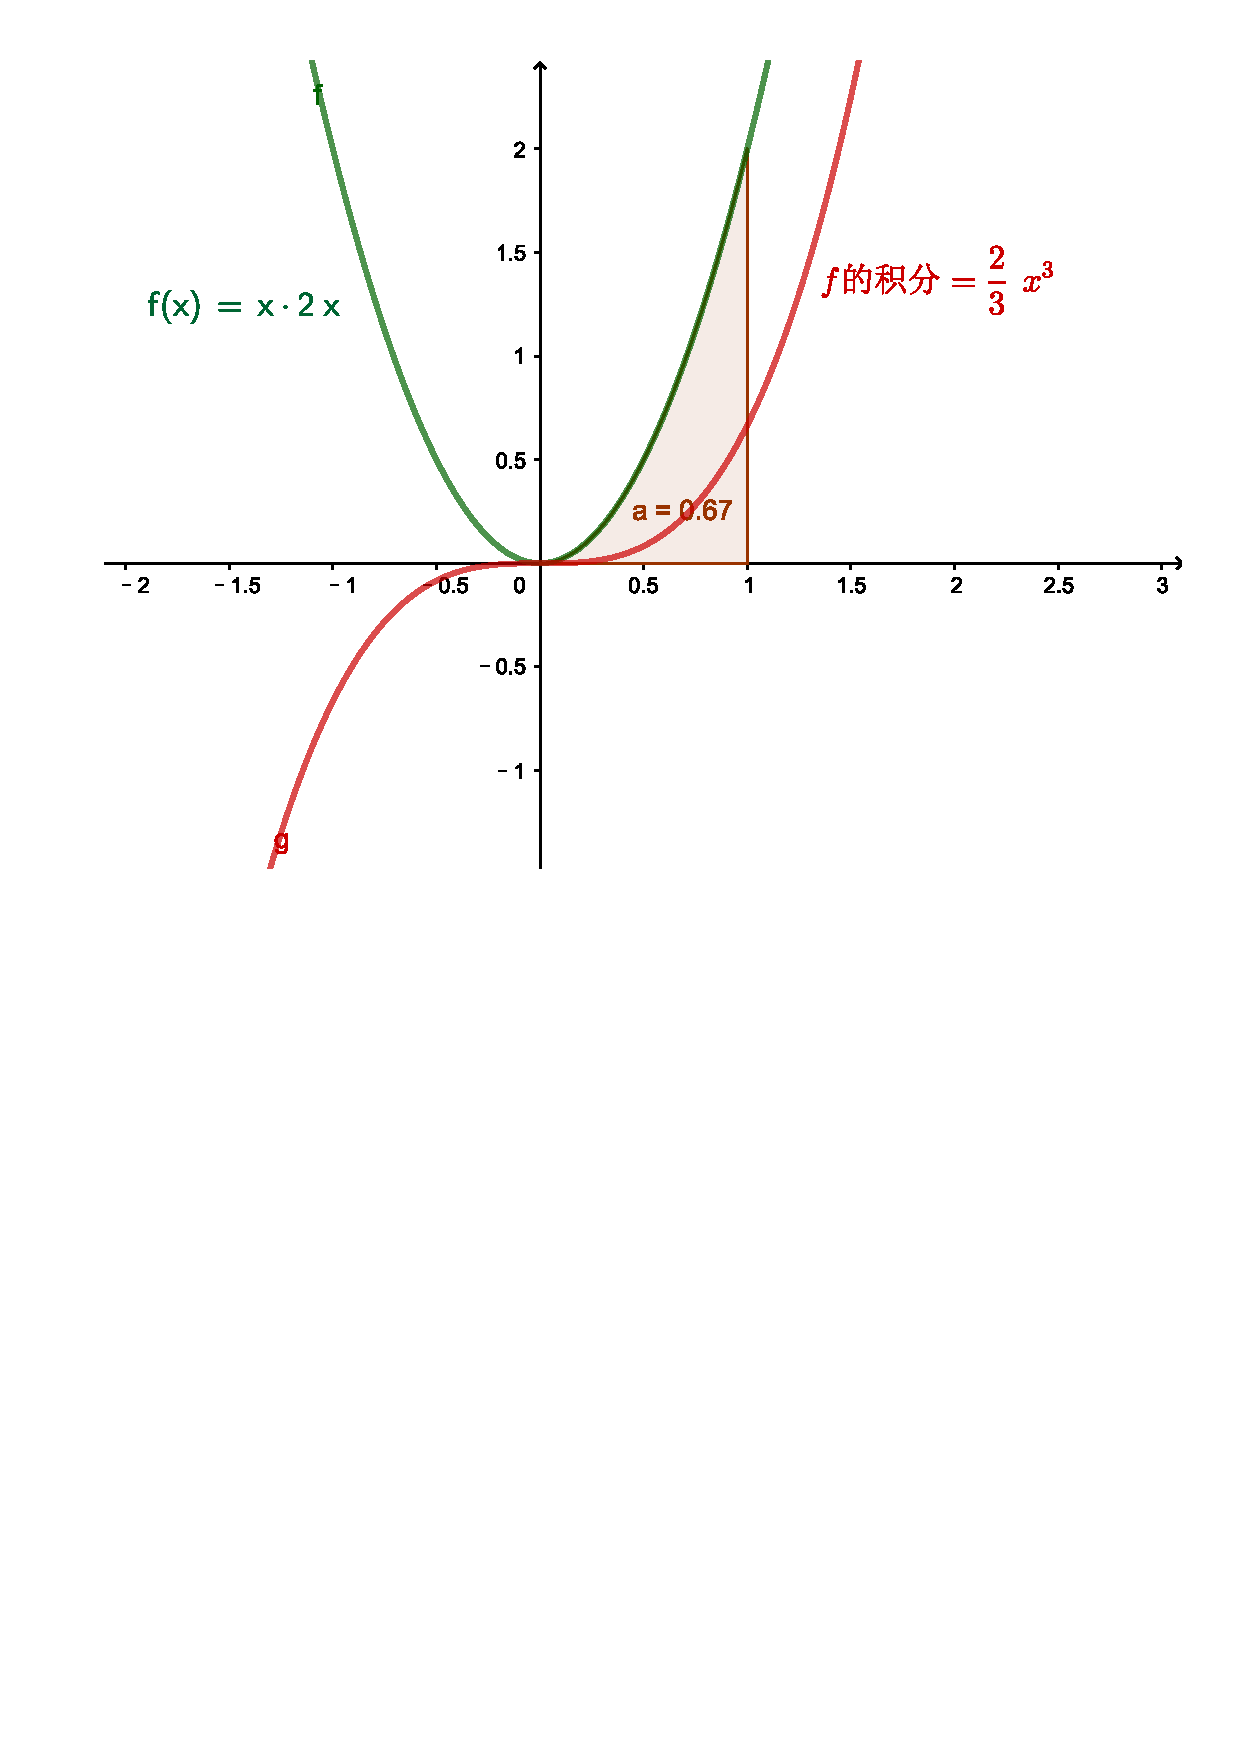
\includegraphics[width=0.5\textwidth]{/0240.pdf} 
\end{myEnvSample}
\vspace{1em} 




\begin{myEnvSample}
	某产品, 根据寿命长短(用随机变量X表示), 分为三档, 每档有不同的定价. \\
	该随机变量X(寿命), 符合$\lambda =\frac{1}{10}$的``指数分布". \\
	(别忘了, 指数分布的``概率函数"公式是: $	f(x)=\left\{ \begin{array}{l}
		\lambda e^{-\lambda x}\ (x\ge 0)\\
		0\ (x<0)\\
	\end{array} \right. 	$) \\

根据寿命 ,分档的价格是:  \\
\begin{tabular}{|c|c|c|c|c|}
	\hline
	寿命(年) & $X \leq 1$ & $1 \leq X \leq 2$ & $2 \leq X \leq 3$ & $X>3$ \\
	\hline
	价格(元) & 1500 & 2000 & 2500 & 3000 \\
	\hline
\end{tabular} \\

我们要先算出, 产品在``每个价格区间"的概率是多少?  因为下面求``价格期望"时, 要用到这些概率数值. \\
$P\{\text{寿命}X\leq 1\text{年\}}=\int_{0\text{年寿命}}^{1\text{年寿命}}{\underset{\text{指数分布的概率函数}f(x)}{\underbrace{\left( \underset{=\frac{1}{10}}{\underbrace{\lambda }}e^{-\lambda x} \right) }}}dx=\int_0^1{\left( \frac{1}{10}e^{-\frac{1}{10}x} \right) dx=0.0952}
$ \\
$P\{1<X\leq 2\}=\int_1^2{\left( \lambda e^{-\lambda x} \right)}dx=\int_0^1{\left( \frac{1}{10}e^{-\frac{1}{10}x} \right) dx=0.0861}
$ \\
$P\{2<X\leq 3\}=\int_2^3{\left( \lambda e^{-\lambda x} \right)}dx=\int_2^3{\left( \frac{1}{10}e^{-\frac{1}{10}x} \right) dx=0.0779}
$ \\
$P\{X>3\}=\int_3^{+\infty}{\left( \lambda e^{-\lambda x} \right)}dx=\int_3^{+\infty}{\left( \frac{1}{10}e^{-\frac{1}{10}x} \right) dx=0.7408}
$ \\

现在就有: \\
\begin{tabular}{|c|c|c|c|c|}
	\hline
	寿命X(年) & (0-1] & (1-2] & (2-3] & >3 \\
	\hline
	价格Y(元) & 1500 & 2000 & 2500 & 3000 \\
	\hline
	概率P & 0.0952 & 0.0861 & 0.0779 & 0.7408 \\
	\hline
\end{tabular} \\

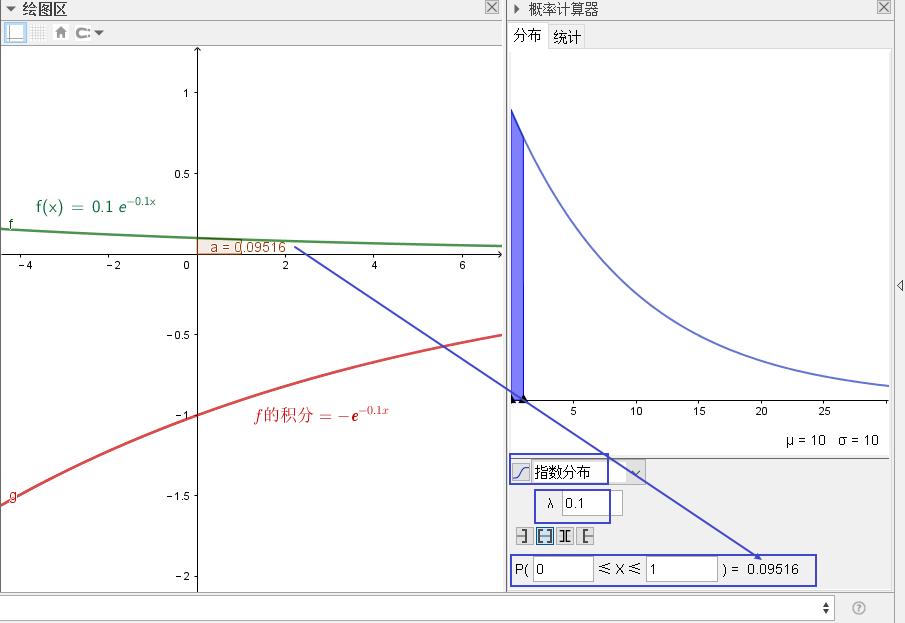
\includegraphics[width=0.7\textwidth]{/0241.png} \\

所以, 该产品的价格期望值, 就是: \\
\begin{align*}  % 支持每行编号. 若不需要编号, 就用 align*环境
	E(\text{价格}Y) & =\left( \underset{\text{``属于该寿命段"产品的价格}}{\underbrace{1500}}\cdot \underset{\text{``会属于该寿命段产品"的概率}}{\underbrace{0.0952}} \right)\\
& +\left( 2000\cdot 0.0861 \right)\\
& +\left( 2500\cdot 0.0779 \right)\\
& +\left( 3000\cdot 0.7408 \right)\\
& =2732.15 \text{元}
\end{align*}
\end{myEnvSample}
	
	
	
\end{document}